\documentclass[journal]{IEEEtran}
\usepackage[utf8]{inputenc}
\usepackage[T1]{fontenc}
\usepackage[spanish,es-noquoting]{babel}
\usepackage{amsmath,amssymb,booktabs,graphicx}
\usepackage[hidelinks]{hyperref}
\graphicspath{{g16_figuras/}}

\title{Evolución temporal de comunidades y polarización política en X}
\author{Sara Valentina Figueredo Laserna y Juan Sebastian Mora Cabrera%
\thanks{Trabajo académico para el curso de Teoría de Grafos.}}
\begin{document}
\maketitle

\begin{abstract}
Las redes sociales digitales constituyen espacios en los que los usuarios producen contenidos, intercambian información y establecen relaciones de interacción. El análisis de estas relaciones mediante la teoría de grafos permite estudiar la estructura de las comunidades y su evolución temporal. Este trabajo propone un modelo de red temporal para examinar las interacciones políticas registradas en X relacionadas con Colombia. Se construyeron grafos dirigidos de respuestas, menciones y citas, representados mediante matrices de adyacencia, y se emplearon matrices laplacianas, agrupamiento espectral y modularidad para estudiar su estructura comunitaria. Se analizaron 37\,069 publicaciones únicas de enero a junio de 2026, obtenidas de 28 exportaciones Zeeschuimer. Las comunidades mostraron bajo solapamiento mensual y la bipartición dependió de las menciones. Al igualar el volumen de publicaciones con interacción se redujo la diferencia de conectividad entre enero y junio, aunque junio siguió presentando la menor fracción de nodos en la componente mayor. Se reconoce que la separación estructural entre comunidades no constituye, por sí sola, evidencia suficiente de polarización ideológica.
\end{abstract}
\begin{IEEEkeywords}
Teoría de grafos, redes temporales, teoría espectral de grafos, polarización política, detección de comunidades, redes sociales.
\end{IEEEkeywords}

\section{Introducción}
Las redes sociales digitales permiten observar diferentes formas de interacción entre usuarios, entre ellas las respuestas, las menciones y las publicaciones citadas. En contextos políticos, estas relaciones pueden utilizarse para estudiar cómo circula la información y cómo se organizan estructuralmente los participantes alrededor de temas, actores o acontecimientos.

La teoría de grafos ofrece herramientas para representar estos sistemas como conjuntos de vértices y aristas. Sin embargo, una red social no debe considerarse necesariamente estática: sus nodos, relaciones y patrones de interacción pueden cambiar con el tiempo. Por esta razón, los modelos de redes temporales permiten incorporar la dimensión cronológica al análisis~\cite{holme}.

Por otra parte, la teoría espectral de grafos estudia las propiedades de un grafo a partir de los valores y vectores propios de matrices asociadas, como la matriz de adyacencia y la matriz laplaciana. Estas herramientas permiten analizar la conectividad y construir métodos de agrupamiento que identifican estructuras comunitarias~\cite{chung,luxburg}.

Este trabajo propone un modelo matemático para estudiar la evolución temporal de comunidades en interacciones políticas relacionadas con Colombia en X. El análisis se plantea a partir de publicaciones recolectadas en distintos momentos y de las relaciones que puedan identificarse de manera verificable en sus metadatos.

El planteamiento inicial distinguía una muestra exploratoria inferior a cien publicaciones de junio a diciembre de 2025 y una ampliación condicional de julio de 2025 a junio de 2026. El corpus efectivamente auditado y utilizado en este artículo abarca enero a junio de 2026. Las cifras y comparaciones del artículo corresponden a ese semestre.

\section{Descripción del problema}
El problema consiste en determinar cómo representar y analizar matemáticamente las relaciones entre cuentas que participan en conversaciones políticas en X y cómo comparar la estructura de esas relaciones a lo largo del tiempo.

Una publicación puede contener menciones a otras cuentas, responder a una publicación previa o citar contenido de otro usuario. Estas acciones no representan necesariamente el mismo tipo de relación. Por ello, deben distinguirse durante la construcción de la red.

La información disponible procede de 28 exportaciones NDJSON de Zeeschuimer, agrupadas inicialmente en carpetas mensuales. La captura incluyó búsquedas sobre Iván Cepeda, Abelardo de la Espriella, Sergio Fajardo y Paloma Valencia. Los archivos contienen identificadores de publicaciones, fechas, autores, texto, menciones y algunos indicadores de respuesta y cita. No obstante, la cobertura depende de las búsquedas efectuadas, de los contenidos que pudieron capturarse y de los metadatos disponibles. En consecuencia, no puede asumirse que la muestra represente la totalidad de la actividad política de X.

El problema se divide en las siguientes preguntas:
\begin{enumerate}
\item ¿Cómo representar las interacciones identificadas como una red dirigida y temporal?
\item ¿Qué propiedades estructurales permiten caracterizar la formación y la separación de comunidades?
\item ¿Cómo pueden utilizarse las matrices laplacianas y sus valores propios para analizar la conectividad y detectar grupos?
\item ¿Cómo comparar las comunidades entre periodos consecutivos?
\item ¿Qué información adicional es necesaria para interpretar la separación estructural como posible polarización política?
\end{enumerate}
La última pregunta es esencial: una red puede presentar comunidades estructuralmente separadas sin que ello demuestre, por sí solo, que sus integrantes sostienen posiciones ideológicas opuestas.

\section{Objetivo general y objetivos específicos}
\subsection{Objetivo general}
Proponer un modelo matemático basado en teoría de grafos y métodos espectrales para analizar la evolución temporal de las comunidades de interacción política en X relacionadas con Colombia, y establecer un procedimiento para estudiar su posible asociación con patrones de polarización política.
\subsection{Objetivos específicos}
\begin{enumerate}
\item Validar la integridad, la cobertura temporal y la disponibilidad de metadatos de la muestra de publicaciones.
\item Representar las relaciones verificables entre cuentas mediante grafos dirigidos, ponderados y etiquetados por tipo de interacción.
\item Construir matrices de adyacencia y matrices laplacianas para analizar las propiedades estructurales de la red.
\item Aplicar un procedimiento de agrupamiento espectral y medidas de modularidad para identificar comunidades.
\item Definir indicadores que permitan comparar la composición y la estructura de las comunidades entre periodos.
\item Establecer criterios para diferenciar la segregación estructural de la polarización ideológica y reconocer las limitaciones de los datos recopilados.
\end{enumerate}

\section{Marco teórico}
\subsection{Grafos dirigidos y ponderados}
Un grafo dirigido se define como
\[
G=(V,E),
\]
donde $V$ es el conjunto de vértices y $E\subseteq V\times V$ es el conjunto de aristas dirigidas.

Un grafo ponderado incorpora una función
\[
w:E\longrightarrow\mathbb R_{>0},
\]
que asigna un peso a cada relación.

\subsection{Redes temporales}
Una red temporal puede representarse mediante una sucesión de grafos
\[
\mathcal G=\{G_1,G_2,\ldots,G_T\},
\]
donde cada $G_t=(V_t,E_t)$ representa las relaciones observadas durante el periodo $t$.

El uso de ventanas temporales permite comparar las redes y estudiar la aparición, persistencia o desaparición de relaciones y grupos. No obstante, los cambios observados también pueden deberse a variaciones en la captura de datos, por lo que la cobertura de cada periodo debe documentarse~\cite{holme}.

\subsection{Matriz de adyacencia}
Sea $G_t$ un grafo con $n_t$ vértices. Su matriz de adyacencia ponderada se define como
\[
A_t=(a^{(t)}_{ij})\in\mathbb R^{n_t\times n_t},
\]
donde $a^{(t)}_{ij}$ representa el peso de las relaciones desde el vértice $i$ hacia el vértice $j$ durante el periodo $t$. En una red dirigida, en general,
\[
a^{(t)}_{ij}\ne a^{(t)}_{ji}.
\]

\subsection{Matriz laplaciana}
Para aplicar el análisis espectral a una red no dirigida y ponderada, se define la matriz de adyacencia simétrica $B_t$ y la matriz diagonal de grados $D_t$, cuyos elementos son
\[
(D_t)_{ii}=\sum_{j=1}^{n_t}(B_t)_{ij}.
\]
La matriz laplaciana combinatoria se define como
\[
L_t=D_t-B_t.
\]
Como $B_t$ es simétrica y tiene pesos no negativos, $L_t$ es simétrica y semidefinida positiva. Sus valores propios pueden ordenarse de la siguiente forma:
\[
0=\lambda_1\le\lambda_2\le\cdots\le\lambda_{n_t}.
\]
La multiplicidad del valor propio cero coincide con el número de componentes conexas del grafo. Cuando la red es conexa, $\lambda_2>0$ (para $n_t\ge 2$). El valor $\lambda_2$, denominado valor propio algebraico de conectividad, aporta información sobre la estructura de conexión del grafo~\cite{chung}.

\subsection{Agrupamiento espectral}
El agrupamiento espectral utiliza los vectores propios de una matriz asociada al grafo para representar sus vértices en un espacio de menor dimensión. Posteriormente, un algoritmo de agrupamiento, como $k$-means, permite asignar los vértices a grupos~\cite{luxburg}. Para una red no dirigida, se puede utilizar la laplaciana normalizada
\[
L_{\mathrm{sym}}=I-D^{-1/2}BD^{-1/2},
\]
cuando los grados son positivos. Los vértices con grado cero requieren un tratamiento específico.

El número de comunidades no debe seleccionarse únicamente para producir una división visualmente atractiva. Debe justificarse mediante criterios estructurales, estabilidad y conocimiento del problema.

\subsection{Modularidad y comunidades}
La modularidad mide, en términos generales, cuánto difiere la cantidad de conexiones internas de una partición respecto de un modelo de referencia. Para una red no dirigida ponderada, una definición habitual es
\[
Q=\frac{1}{2m}\sum_{i,j}\left(B_{ij}-\frac{k_i k_j}{2m}\right)\delta(c_i,c_j),
\]
donde $k_i=\sum_j B_{ij}$, $2m=\sum_i k_i$, $c_i$ es la comunidad del vértice $i$ y $\delta(c_i,c_j)$ vale uno si ambos vértices pertenecen a la misma comunidad, y cero en otro caso~\cite{newman}.

Una modularidad elevada puede sugerir una estructura comunitaria marcada respecto del modelo de referencia. Sin embargo, no demuestra que los grupos correspondan a ideologías políticas distintas.

\subsection{Polarización política y segregación estructural}
En este trabajo se distingue entre dos conceptos. La segregación estructural se refiere a la concentración de interacciones dentro de determinados grupos y a la escasez relativa de conexiones entre ellos. La polarización ideológica implica diferencias sustantivas entre las posiciones políticas de los participantes.

Las propiedades topológicas permiten estudiar la primera dimensión. Para examinar la segunda se requiere evidencia adicional, como etiquetas ideológicas justificadas mediante fuentes verificables o un procedimiento de análisis de contenido validado. Por tanto, las métricas de modularidad, conectividad o agrupamiento espectral se interpretarán como indicadores de estructura de red, no como medidas directas y suficientes de ideología.

\section{Modelamiento del problema}
\subsection{Conjunto de cuentas y periodos}
Para cada periodo se define el grafo
\[
G_t=(V_t,E_t,W_t),
\]
donde $V_t\subseteq U$ contiene las cuentas identificadas en ese periodo, $E_t$ contiene las relaciones observadas y $W_t$ asigna sus pesos. Sea $U$ el conjunto de cuentas identificadas en las publicaciones recopiladas. Se considera una secuencia de periodos mensuales $\mathcal T=\{t_1,\ldots,t_T\}$.

En el contexto de este trabajo, cada vértice representa una cuenta identificada en los datos y una arista $(u,v)$ representa una relación observada desde la cuenta $u$ hacia la cuenta $v$. Por ejemplo, una respuesta de $u$ a una publicación de $v$ puede representarse mediante una arista $u\to v$. Si varias interacciones del mismo tipo se producen entre dos cuentas durante un periodo, el peso puede representar su frecuencia.

Para esta investigación se emplearon ventanas mensuales. Así, cada publicación se asignó al mes correspondiente a su marca temporal en Bogotá (UTC$-5$) y cada relación se incorporó al grafo del periodo en el que fue observada. Se usó el identificador estable, preservado como texto. Los nombres de usuario solos quedaron como posible alternativa del diseño inicial. En la implementación, las aristas requieren un identificador verificable en ambos extremos.

\subsection{Representación de las interacciones}
Sea $R=\{r_1,\ldots,r_s\}$ el conjunto de tipos de relación considerados, por ejemplo, respuestas, menciones y citas. Para cada periodo $t$ y relación $r$, se define
\[
A^{(r)}_t=(a^{(t,r)}_{ij}),
\]
donde $a^{(t,r)}_{ij}$ es el número de interacciones observadas de tipo $r$ desde la cuenta $i$ hacia la cuenta $j$ durante $t$.

La matriz puede construirse por tipo de interacción. Por ejemplo, $A^{(r)}_t$ representa las respuestas cuando $r$ es la etiqueta de respuesta, mientras que $A^{(m)}_t$ representa las menciones. Esta separación permite analizar cada relación individualmente antes de combinarlas. Las menciones, respuestas y citas deben conservarse como tipos de relación diferentes, pues una mención no implica necesariamente una conversación directa.

Se propone una matriz dirigida agregada:
\[
W_t=\sum_{r\in R}\alpha_r A^{(r)}_t,\qquad \alpha_r\ge 0,
\]
donde $\alpha_r$ representa el peso asignado a cada tipo de interacción. Los coeficientes no se fijarán arbitrariamente para favorecer una conclusión. En el análisis inicial se mantuvieron separadas las matrices por tipo de relación. La referencia agregada asignó $\alpha_r=1$ por evento verificado, con una unidad como máximo por publicación, tipo y destinatario. Las capas se contrastaron también con ponderaciones alternativas. Los autolazos quedaron en el registro de eventos y se excluyeron de las matrices.

Las métricas espectrales no dirigidas se calcularán, si resulta apropiado, sobre la matriz simétrica
\[
B_t=\frac{W_t+W_t^{\mathsf T}}{2}.
\]
Esta transformación permite utilizar herramientas espectrales para grafos no dirigidos, pero elimina la distinción entre la dirección de las interacciones. Por ello, se conservará también la red dirigida original para describir las relaciones.

\subsection{Matrices y propiedades estructurales}
A partir de $B_t$, se define
\[
D_t=\operatorname{diag}\left(\sum_j (B_t)_{1j},\ldots,\sum_j (B_t)_{n_tj}\right)
\]
y $L_t=D_t-B_t$.

Se estudiarán el número de vértices, el número de aristas, la distribución de grados, las componentes conexas y los valores propios de $L_t$. La interpretación de $\lambda_2$ se realizará considerando la conectividad de cada grafo: si el grafo es desconectado, $\lambda_2=0$ y no debe interpretarse como si describiera una red conexa. Para comparar periodos con diferentes tamaños se considerará también la laplaciana normalizada, cuando las condiciones matemáticas de su definición se satisfagan.

La implementación usó $S_t=W_t+W_t^{\mathsf T}=2B_t$. En vértices de grado positivo, sustituir $B_t$ por $2B_t$ deja invariante $D_t^{-1/2}B_tD_t^{-1/2}$. También deja invariante la modularidad ponderada, pues todos los pesos y el peso total se multiplican por el mismo factor. En el laplaciano combinatorio sí se duplica la escala de los autovalores. Se reportan autovalores normalizados en la componente mayor (CM).

\subsection{Detección de comunidades}
En cada periodo se aplicará un procedimiento de agrupamiento espectral a la matriz laplaciana apropiada. Los vectores propios asociados a los valores propios seleccionados se utilizarán como representación de los vértices y, posteriormente, se realizará el agrupamiento.

Las particiones se contrastarán mediante modularidad y mediante la inspección de su estabilidad ante cambios razonables de parámetros. El número de comunidades y los parámetros del algoritmo se tratarán como decisiones exploratorias, no como valores conocidos de antemano.

\subsection{Comparación temporal}
Sea $\mathcal C_t$ el conjunto de comunidades detectadas en el periodo $t$. Para comparar dos comunidades $C_i^{(t)}$ y $C_j^{(t+1)}$, se propone utilizar el índice de Jaccard:
\[
J(C_i^{(t)},C_j^{(t+1)})=
\frac{|C_i^{(t)}\cap C_j^{(t+1)}|}{|C_i^{(t)}\cup C_j^{(t+1)}|}.
\]
Un valor alto indica una mayor coincidencia entre los conjuntos de cuentas identificadas en ambos periodos. El índice debe interpretarse con cuidado si cambia la cobertura de la muestra o si las cuentas no aparecen en todos los meses.

Se compararán además los tamaños de las comunidades, la modularidad, la conectividad y el número de relaciones entre grupos. Estas comparaciones describirán cambios en la muestra observada y no necesariamente cambios de toda la población de usuarios de X.

\subsection{Operacionalización de la polarización}
La polarización no se definirá exclusivamente a partir de la modularidad. Como análisis complementario, si se obtienen clasificaciones políticas justificables, se estudiará la proporción de relaciones que conectan cuentas asignadas a grupos diferentes. Para una red no dirigida, una medida descriptiva posible es
\[
P_t=1-\frac{\sum_{i,j}B_{ij}\mathbf{1}[g_i\ne g_j]}{\sum_{i,j}B_{ij}},
\]
donde $g_i$ representa la categoría política asignada a la cuenta $i$ y $\mathbf 1[\cdot]$ es la función indicadora.

Con esta convención, valores mayores indican una mayor proporción del peso de las aristas dentro de categorías políticas iguales. La medida solo podrá calcularse si las categorías tienen una definición independiente y verificable y si el denominador es positivo. No se calculará a partir de comunidades inferidas por el mismo algoritmo sin reconocer el carácter circular de esa interpretación.

\section{Solución propuesta}
La solución se organiza en cinco etapas.

\subsection{Etapa 1: validación de los datos}
Se comprobó la integridad de 28 archivos NDJSON de Zeeschuimer mediante el manifiesto SHA-256 y se auditó la presencia de identificadores, la validez de las fechas, los duplicados y la disponibilidad de campos de interacción. Los identificadores se conservaron como texto para evitar pérdida de precisión. De 39\,787 registros quedaron 37\,069 publicaciones únicas dentro de enero a junio de 2026. La auditoría conservó la procedencia por archivo y línea y registró la fecha real en Bogotá. Los materiales de análisis agregado omiten campos personales innecesarios.

\subsection{Etapa 2: construcción de redes}
Las relaciones se extrajeron de forma separada según su tipo. Las respuestas se identificaron mediante sus metadatos, las menciones mediante entidades del texto y las citas mediante el autor anidado o la búsqueda de la publicación citada por ID. Las republicaciones quedaron sin aristas por falta de referencias estructuradas. Los contadores agregados de respuestas, retuits, citas o me gusta no se utilizaron como relaciones individuales. Se corroboró una muestra de eventos contra las capturas originales.

\subsection{Etapa 3: análisis espectral}
Se construyeron las matrices de adyacencia por periodo y las laplacianas normalizadas de las componentes mayores. Se examinaron los valores propios, la conectividad y la estabilidad de las particiones. Para componentes de hasta 256 nodos se empleó diagonalización densa y para las mayores se usó una aproximación de Ritz. La bipartición se obtuvo con los primeros dos autovectores normalizados por fila y $k$-medias con 20 reinicios. Como contraste se aplicaron fusiones voraces por ganancia positiva de modularidad, con un número de grupos determinado por el algoritmo.

\subsection{Etapa 4: análisis temporal}
Las comunidades se compararon entre periodos mediante Jaccard y el índice de Rand ajustado (ARI)~\cite{hubert}, calculado sobre las cuentas comunes cuando la comparación era informativa. También se examinaron cambios en los nodos, las aristas, la modularidad y la conectividad. Se hizo una comprobación de sensibilidad a los pesos y se igualó el número de publicaciones con interacción, muestreando publicaciones completas y conservando sus eventos. Se añadieron comparaciones descriptivas de calendario y contenido.

\subsection{Etapa 5: interpretación y limitaciones}
La interpretación distinguirá los resultados topológicos de las conclusiones ideológicas. La existencia de comunidades, una modularidad elevada o una conectividad reducida entre grupos se considerará evidencia de estructura relacional, no una demostración automática de polarización política. El intervalo julio de 2025 a junio de 2026 estaba condicionado a disponer de capturas comparables. Los resultados se restringen al corpus de enero a junio de 2026.

\section{Resultados}
\subsection{Cobertura y verificación}
Las 28 capturas coincidieron con el manifiesto. De 39\,787 filas, 2\,667 fueron copias adicionales y 51 publicaciones únicas quedaron fuera del intervalo. Hubo 458 filas cuyo mes de publicación no coincidió con el mes de la carpeta. El 2 de mayo y el 27 de junio quedaron sin publicaciones observadas. La Tabla~\ref{tab:estructura} muestra las diferencias de cobertura y tamaño.

Se resolvieron 43\,901 eventos: 11\,197 respuestas, 2\,951 citas y 29\,753 menciones, con un conteo por destinatario y publicación dentro de cada tipo. Quedaron 135 citas sin destinatario verificable. Se excluyeron 764 autolazos de las matrices. La agregación por par dirigido, mes y tipo produjo 35\,832 aristas. Las sumas de las capas cuentan por separado los eventos de una publicación que también corresponden a otro tipo.

Se corroboraron 42 eventos contra los originales: 12 respuestas, 12 menciones, 12 citas directas y los seis casos de cita resueltos por búsqueda en el corpus. La revisión temática de ocho textos por mes encontró 32 electorales explícitos, 12 de política sin vínculo electoral explícito, tres con contexto insuficiente y uno fuera de tema. La muestra balanceada por mes tiene una sola codificación por texto y no estima la prevalencia temática del corpus completo.

\begin{table*}[t]
\centering
\caption{Red agregada dirigida y componente mayor. La reciprocidad usa arcos distintos y la concentración usa el peso entrante. El autovalor pertenece a la laplaciana normalizada de la CM.}
\label{tab:estructura}
\begin{tabular}{lrrrrrrrrr}
\toprule
Mes & Publicaciones & Días & Nodos & Arcos & Comp. & CM (\%) & $\lambda_2$ CM & Recip. (\%) & Peso 10 destinos (\%)\\
\midrule
Ene. & 16\,149 & 31/31 & 5\,822 & 13\,512 & 141 & 94,2 & 0,03027 & 0,64 & 28,1\\
Feb. & 9\,231 & 28/28 & 3\,234 & 6\,649 & 94 & 93,5 & 0,02745 & 0,90 & 32,3\\
Mar. & 4\,241 & 31/31 & 1\,454 & 2\,247 & 81 & 87,4 & 0,02280 & 1,69 & 33,3\\
Abr. & 4\,153 & 30/30 & 1\,345 & 2\,168 & 69 & 85,4 & 0,02536 & 1,57 & 34,6\\
May. & 1\,855 & 30/31 & 735 & 848 & 66 & 77,6 & 0,01598 & 2,83 & 36,1\\
Jun. & 1\,440 & 29/30 & 599 & 607 & 95 & 59,9 & 0,01241 & 0,99 & 31,0\\
\bottomrule
\end{tabular}
\end{table*}

\subsection{Familia de grafos y sensibilidad al volumen}
Se verificaron 30 adyacencias y 30 laplacianas normalizadas de la componente mayor, incluidas las capas vacías. Las 24 redes no vacías estaban desconectadas, de modo que la multiplicidad del cero y el tamaño de la componente mayor aportan información que el segundo autovalor global no distingue. Los dos primeros pares propios de las componentes mayores satisfacieron un umbral de residual de $10^{-7}$. El $\lambda_2$ normalizado de la red agregada bajó de 0,03027 en enero a 0,01241 en junio, con un repunte local en abril.

La reciprocidad se define como la fracción de arcos distintos $(i,j)$ que tienen arco inverso $(j,i)$ en el mismo mes. En la red agregada se mantuvo entre 0,64 y 2,83\,\%. La fracción del peso total recibido por los diez destinatarios principales fue del 28,1 al 36,1\,\%. Una componente conectada puede contener muchos caminos entre cuentas aunque pocas parejas interactúen en ambos sentidos y el peso se concentre en pocos destinos. Esta diferencia justifica mantener la dirección para el diagnóstico y usar la simetrización para el espectro.

En la Fig.~\ref{fig:conectividad}, la estructura de menciones se aproxima a la agregada, mientras las respuestas se fragmentan de forma más marcada. En mayo su componente mayor contiene 26 de 340 cuentas y en junio 10 de 255. Agrupar todos los tipos oculta esa diferencia. En junio, solo 359 de 599 nodos de la red agregada pertenecen a la componente mayor, por lo que las particiones de ese mes dejan fuera a 240 nodos.

\begin{figure}[t]
\centering
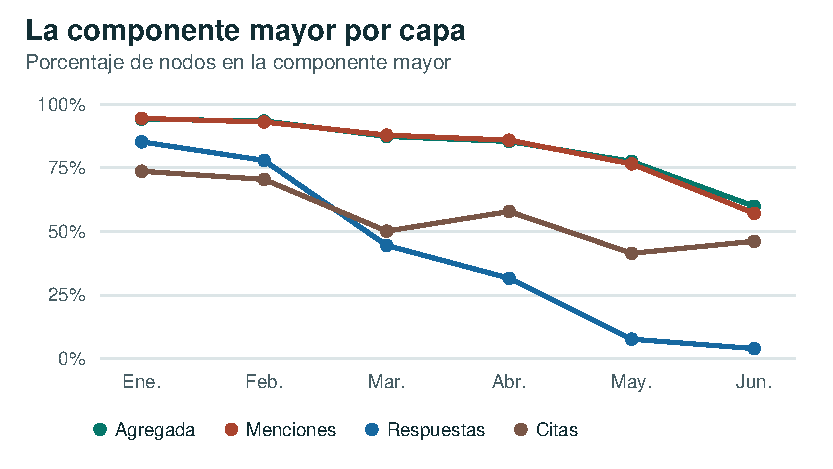
\includegraphics[width=\columnwidth]{conectividad.pdf}
\caption{Fracción de nodos en la componente mayor de cada capa no vacía.}
\label{fig:conectividad}
\end{figure}

Para evaluar cuánto puede influir el volumen, se hicieron 120 extracciones sin reemplazo de 433 publicaciones por mes entre las que tenían al menos un evento no reflexivo. Se mantuvieron juntos los eventos de cada publicación. Junio fija ese mínimo y siempre se incluye completo. Con todos los datos, la diferencia de la componente mayor entre enero y junio es de 34,2 puntos porcentuales. Con el tamaño igualado, la mediana de enero baja a 70,6\,\% frente al 59,9\,\% de junio, una brecha de 10,6 puntos. Las restantes medianas entre febrero y mayo se sitúan entre 73,0 y 75,6\,\%. Junio quedó por debajo del percentil 5 de las submuestras de cada mes anterior. El volumen modifica sustancialmente el contraste. La brecha residual puede reflejar diferencias en la composición y en la captura. Los percentiles resumen las submuestras de los datos disponibles y no son intervalos de inferencia poblacional.

\begin{figure}[t]
\centering
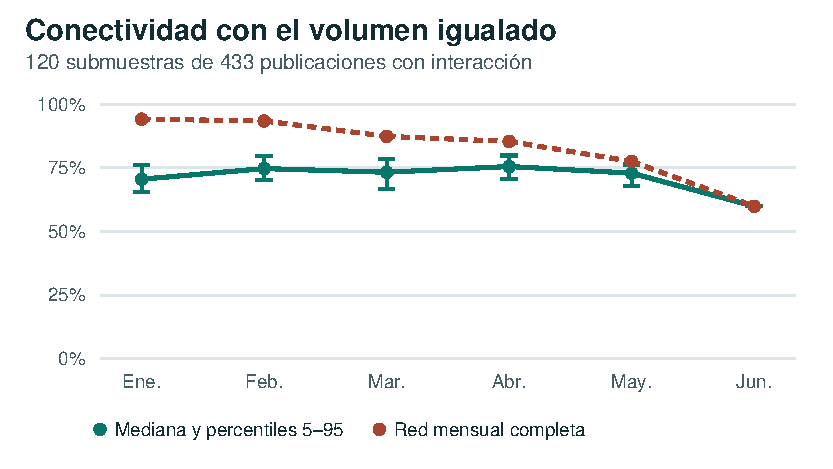
\includegraphics[width=\columnwidth]{volumen.pdf}
\caption{Comparación de la red completa con submuestras del mismo número de publicaciones con interacción.}
\label{fig:volumen}
\end{figure}

\subsection{Comunidades y particiones}
En la red agregada, la bipartición espectral separa un grupo de 8 a 21 cuentas. Su modularidad va de 0,0011 a 0,0573. Es compatible con cortes locales en la componente mayor y no sustenta una lectura de dos bloques comparables. Las respuestas ofrecieron cortes más equilibrados en febrero (610 frente a 1\,054 cuentas) y abril (96 frente a 104), con $Q=0,412$ y $Q=0,486$, respectivamente. La fragmentación de esta capa reduce el universo al que se pueden atribuir esos cortes.

\begin{table}[t]
\centering
\caption{Particiones de la componente mayor agregada}
\label{tab:particiones}
\begin{tabular}{lrrrr}
\toprule
Mes & Grupo menor$^a$ & $Q^a$ & Grupos$^b$ & $Q^b$\\
\midrule
Ene. & 11 & 0,0011 & 79 & 0,5351\\
Feb. & 9 & 0,0020 & 60 & 0,5859\\
Mar. & 10 & 0,0083 & 38 & 0,6685\\
Abr. & 21 & 0,0212 & 36 & 0,5998\\
May. & 8 & 0,0238 & 29 & 0,7299\\
Jun. & 16 & 0,0573 & 27 & 0,7126\\
\bottomrule
\end{tabular}\\
\footnotesize $^a$ Bipartición espectral. $^b$ Fusión voraz por modularidad.
\end{table}

El método voraz produjo de 27 a 79 grupos y $Q$ de 0,535 a 0,730 en la capa agregada (Tabla~\ref{tab:particiones}). El ARI entre los dos métodos fue de 0,0003 a 0,0181. La optimización tiene objetivos y resoluciones diferentes de los de la bipartición. Un $Q$ mayor del método que optimiza esa función es esperable. Estos $Q$ son descriptivos y no se contrastaron contra una distribución nula. Su interpretación también depende de la resolución del método~\cite{fortunato}. El tratamiento por capas es coherente con representar interacciones distintas antes de agregarlas, aunque aquí las capas se analizaron separadamente en lugar de acoplar sus particiones~\cite{mucha}.

En la red agregada, el máximo Jaccard de cada transición fue 0,134--0,228 para la bipartición y 0,083--0,222 para la fusión voraz, tomando los conjuntos completos. Al restringir el método voraz a las cuentas compartidas en ambas componentes mayores, los mejores Jaccard subieron a 0,292--0,500. Eso muestra que pueden persistir subconjuntos locales aun cuando cambian muchas cuentas. La coincidencia conjunta de las particiones sigue siendo baja: el ARI sobre cuentas comunes fue 0,034--0,103. Las cuentas compartidas bajaron de 1\,586 en enero--febrero a 113 en mayo--junio (Fig.~\ref{fig:persistencia}). Jaccard máximo mide el mejor par de comunidades y el ARI evalúa la asignación conjunta sobre el conjunto compartido. La diferencia entre ambos ayuda a distinguir persistencia local de continuidad global.

\begin{figure}[t]
\centering
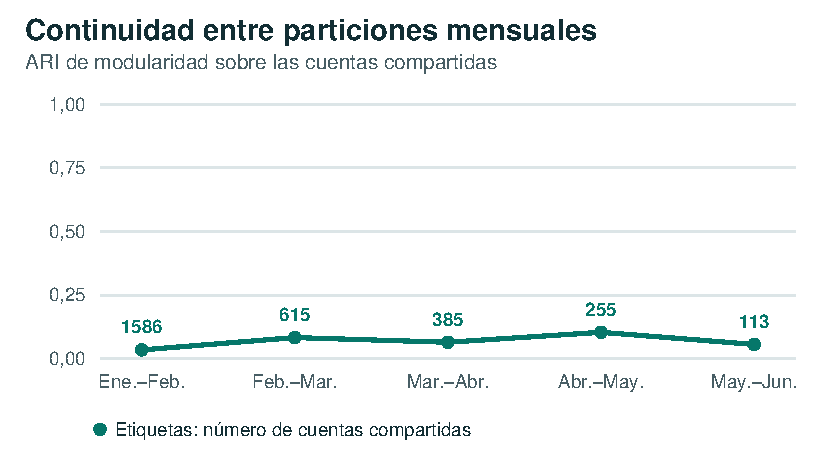
\includegraphics[width=\columnwidth]{persistencia.pdf}
\caption{ARI mensual para las particiones de modularidad sobre las cuentas presentes en ambas componentes mayores.}
\label{fig:persistencia}
\end{figure}

Duplicar el peso de las respuestas o de las citas mantuvo el ARI entre 0,890 y 1,000 respecto de la bipartición de referencia. Excluir las menciones produjo cinco ARI cercanos a cero. En mayo, la intersección no conservó ambos grupos en al menos una de las particiones. Binarizar pesos cambió la bipartición agregada en cuatro meses. Estos contrastes separan una modificación moderada de pesos de una modificación en la definición de las relaciones.

\subsection{Texto y contexto electoral}
Se seleccionó el texto más largo disponible por publicación deduplicada, se retiraron URL y se normalizaron mayúsculas y tildes. Se aplicaron reglas explícitas que detectan nombres completos o identificadores textuales de las cuatro figuras y palabras clave de cinco temas. Una publicación puede coincidir con varias categorías. El denominador es el total de textos del mes. Las reglas detectan coincidencias léxicas y no fueron calibradas para estimar el tema de cada publicación. Los resultados pueden omitir sinónimos, imágenes, ironía o referencias implícitas.

\begin{figure}[t]
\centering
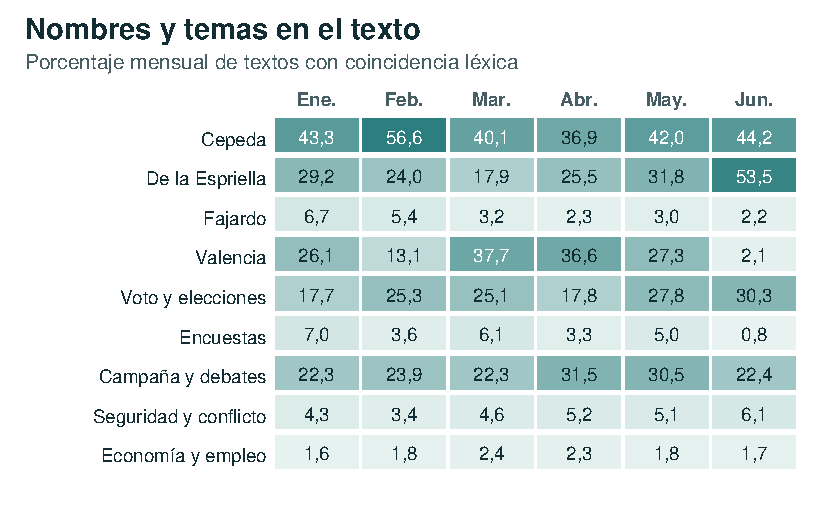
\includegraphics[width=\columnwidth]{contenido.pdf}
\caption{Porcentaje de publicaciones con coincidencias léxicas por figura y tema. Las categorías se superponen.}
\label{fig:contenido}
\end{figure}

En total, 33\,770 textos (91,1\,\%) coincidieron con al menos una figura y 3\,464 (9,3\,\%) con dos o más. Este nivel de presencia debe leerse en el contexto de las búsquedas de origen. Paloma Valencia pasó de aparecer en el 37,7\,\% de marzo al 2,1\,\% de junio. De la Espriella pasó del 17,9 al 53,5\,\% en esos meses. Cepeda se mantuvo por encima del 36\,\% todos los meses. Las coincidencias con voto y elecciones fueron 17,7\,\% en enero y 30,3\,\% en junio. Las de campaña y debates alcanzaron 31,5\,\% en abril. En junio, seguridad y conflicto coincidió con 55 de 771 textos que nombraban a De la Espriella (7,1\,\%) y con 37 de 636 que nombraban a Cepeda (5,8\,\%). Las bases pueden solaparse. Las comparaciones son coocurrencias en el texto capturado y dejan abierta la interpretación de apoyo o crítica.

Como análisis complementario, se calculó TF-IDF por autor y mes y similitud coseno en los grupos con suficiente texto. Se requirieron cinco publicaciones utilizables en español por autor y cinco autores elegibles por grupo. El grupo pequeño de la bipartición solo tuvo de cero a tres autores elegibles. En las dos comunidades mayores de modularidad el umbral se cumplió los seis meses. El coseno medio entre grupos fue menor que ambos promedios internos de enero a mayo. En junio, el promedio entre grupos fue 0,155 y los internos fueron 0,153 y 0,211. Esta comparación describe el vocabulario de una fracción activa de las cuentas y no estima significancia estadística.

Se documentaron los conteos anterior, durante y posterior a tres hitos oficiales~\cite{registraduria}. En torno al 8 de marzo se observaron 863, 766 y 956 publicaciones. En la primera vuelta del 31 de mayo se observaron 211, 184 y 320. En la segunda vuelta del 21 de junio se observaron 325, 192 y 299. Las ventanas laterales duran siete días y la jornada dura uno. En la última ventana posterior un día quedó sin registros. Las diferencias son descriptivas y no identifican un efecto causal de las jornadas.

\section{Discusión y conclusiones}
La familia de grafos muestra diferencias que se pierden al mirar únicamente la red agregada. Las menciones acompañan su conectividad y explican parte de la estabilidad de su bipartición ante cambios moderados de peso. Las respuestas se fragmentan más y ofrecen cortes equilibrados solo en algunos periodos. La comparación a volumen igualado reduce la diferencia entre enero y junio, y hace visible cuánto depende la conectividad del volumen de publicaciones con interacción.

La poca continuidad de las particiones tiene dos componentes: la rotación de cuentas y los cambios de agrupamiento entre las que permanecen. El ARI de modularidad sobre el conjunto compartido sigue bajo incluso al controlar la primera de esas dimensiones. El análisis léxico documenta un cambio en la presencia relativa de las figuras buscadas y la frecuencia de vocabulario electoral. Estos indicadores describen el corpus y no identifican comunidades ideológicas ni un cambio causal de la polarización.

Para estimar $P_t$ serían necesarias categorías políticas independientes, cobertura suficiente de esas etiquetas, acuerdo entre revisores y un referente que considere tamaños y grados de los grupos. La revisión muestral corrobora aristas observadas y no mide interacciones omitidas. El código y tablas agregadas permiten reproducir la auditoría, las particiones, los contrastes y las figuras sin distribuir publicaciones ni identificadores.

\section{Bibliografía}
\begin{thebibliography}{8}
\bibitem{holme} P. Holme y J. Saramäki, \emph{Temporal networks}, Physics Reports, vol. 519, no. 3, pp. 97--125, 2012. doi: 10.1016/j.physrep.2012.03.001.
\bibitem{chung} F. R. K. Chung, \emph{Spectral Graph Theory}. Providence, RI, EE. UU.: American Mathematical Society, 1997.
\bibitem{luxburg} U. von Luxburg, \emph{A tutorial on spectral clustering}, Statistics and Computing, vol. 17, no. 4, pp. 395--416, 2007. doi: 10.1007/s11222-007-9033-z.
\bibitem{newman} M. E. J. Newman, \emph{Modularity and community structure in networks}, Proceedings of the National Academy of Sciences, vol. 103, no. 23, pp. 8577--8582, 2006. doi: 10.1073/pnas.0601602103.
\bibitem{mucha} P. J. Mucha, T. Richardson, K. Macon, M. A. Porter y J.-P. Onnela, \emph{Community structure in time-dependent, multiscale, and multiplex networks}, Science, vol. 328, no. 5980, pp. 876--878, 2010. doi: 10.1126/science.1184819.
\bibitem{fortunato} S. Fortunato, \emph{Community detection in graphs}, Physics Reports, vol. 486, nos. 3--5, pp. 75--174, 2010. doi: 10.1016/j.physrep.2009.11.002.
\bibitem{hubert} L. Hubert y P. Arabie, \emph{Comparing partitions}, Journal of Classification, vol. 2, pp. 193--218, 1985.
\bibitem{registraduria} Registraduría Nacional del Estado Civil, \emph{Elecciones 2026}. \url{https://www.registraduria.gov.co/-Elecciones-2026-.html}.
\end{thebibliography}
\end{document}
